\documentclass[english,compress]{beamer}
\usepackage{kloeckislides}
\nonstopmode

\usepackage[normalem]{ulem}
\usepackage{pifont}
\usepackage{ifthen}

\setbeamercolor{section in head/foot}{use=structure,bg=structure.fg!25!bg}
\defbeamertemplate*{footline}{split theme}
{%
  \leavevmode%
  \begin{beamercolorbox}[wd=.5\paperwidth,ht=2.5ex,dp=1.125ex]{section in head/foot}%
    \insertsectionnavigationhorizontal{\paperwidth}{\hskip0pt plus1filll}{}%
  \end{beamercolorbox}%
  %\begin{beamercolorbox}[wd=.5\paperwidth,ht=2.5ex,dp=1.125ex]{subsection in head/foot}%
    %\insertsubsectionnavigationhorizontal{.5\paperwidth}{}{\hskip0pt plus1filll}%
  %\end{beamercolorbox}%
}


%\useoutertheme[subsection=false]{miniframes}

\setbeamertemplate{frametitle}[default][center]

\AtBeginDocument{%
  {
    \usebeamercolor{section in head/foot}
  }
  
  \pgfdeclareverticalshading{beamer@headfade}{\paperwidth}
  {%
    color(0cm)=(bg);
    color(1.25cm)=(section in head/foot.bg)%
  }

  \setbeamercolor{section in head/foot}{bg=}
}

\addtoheadtemplate{\pgfuseshading{beamer@headfade}\vskip-1.25cm}{}

\beamertemplatedotitem

\setbeamercolor{section in head/foot}{parent=palette quaternary}
\setbeamercolor{subsection in head/foot}{parent=palette primary}

\setbeamercolor{author in head/foot}{parent=section in head/foot}
\setbeamercolor{title in head/foot}{parent=subsection in head/foot}



\AtBeginSection[] {
  \begin{frame}<beamer>
  \frametitle{Outline}
  \tableofcontents[sectionstyle=show/shaded,subsectionstyle=show/show/hide]
\end{frame}
}
\AtBeginSubsection[] {
  \begin{frame}<beamer>
  \frametitle{Outline}
  \tableofcontents[sectionstyle=show/shaded,subsectionstyle=show/shaded/hide]
\end{frame}
}

\newcommand{\technicality}[2]{%
  {\strut #1\\
    \begin{beamercolorbox}[sep=1mm]{block body}
      #2
    \end{beamercolorbox}
  }%
}

\lstset{
  language=C++,
  rangebeginprefix=//\ ,
  rangeendprefix=//\ ,
}

\def\weblink#1#2{\href{#1}{\color{blue}\underline{#2}}}

\definecolor{fetch}{RGB}{227,110,35}
\definecolor{alu}{RGB}{255,188,24}
\definecolor{context}{RGB}{132,146,175}

\usepackage{keystroke}

\setbeamertemplate{navigation symbols}{}

\def\hilite<#1>#2{\alt<#1>{\colorbox{blue!30}{#2}}{\colorbox{white}{#2}}%
}

\lstset{
  language=C++,
  rangebeginprefix=//\ ,
  rangeendprefix=//\ ,
}

\colorlet{input}{green!30}
\colorlet{output}{red!30}
\colorlet{intermed}{blue!30}

\tikzset{
  input/.style={circle,fill=input,draw,thick,minimum height=4.5ex},
  output/.style={circle,fill=output,draw,thick,minimum height=4.5ex},
  func/.style={->,thick},
}

\begin{document}
% {{{ front matter

\title{High-Performance Scientific Computing\\Lecture 11: GPU Performance, Applications}

\date{MATH-GA 2011 / CSCI-GA 2945 $\cdot$ November 21, 2012}

\frame{\titlepage}

\begin{frame}{Today}
  \tableofcontents[hideallsubsections]
\end{frame}
% }}}
% -----------------------------------------------------------------------------
\begin{comment}
\begin{frame}{Bits and pieces}
  \begin{itemize}
    \item Don't have a project? Let's fix that \emph{very soon}
    \item HW5: soon
    \item HW6: due today
    \item Dec 5: Last day of regular class
    \item Dec 12: Legislative Day
    \item Dec 17/18/\textbf{19}: Project presentations
    \item Don't have grade reports for HW1\dots4? Talk to me
  \end{itemize}
\end{frame}
\end{comment}

\begin{comment}
% -----------------------------------------------------------------------------
\section[Version Control]{Tool of the day: Advanced Version Control}
% -----------------------------------------------------------------------------
% {{{
\begin{frame}{Git tricks}
  \begin{center}
  \Huge Version control demo time
  \end{center}
\end{frame}
% }}}
\end{comment}
% -----------------------------------------------------------------------------
\section{GPU performance}
% -----------------------------------------------------------------------------
% {{{
% -----------------------------------------------------------------------------
\subsection{Understanding GPUs}
% -----------------------------------------------------------------------------
\begin{frame}{Comparing architectures}
  \begin{tabular}{l|cccc|l}
    & GF100 & GF104 & GK104 & GCN & Units\\
    \hline
    \# Warps/Wavefronts & 48 & 48 & 64 & 40 \\
    Warp Size & 32 & 32 & 32 & 64 & W.Item \\
    \hline
    SP FLOP/clock & 64 & 96 & 384 & 128 \\
    Clock & 700 & 650 & 823 & 925 & MHz \\
    \hline
    Reg File & 128 & 128 & 256 & 256 & kiB \\
    Lmem & 64  & 64 & 64 & 64 & kiB \\
    Lmem BW & 64  & 64 & 128 & 128 & B/clock \\
    \hline
  \end{tabular}
  \creditto{David Kanter / Realworldtech.com}
\end{frame}
% -----------------------------------------------------------------------------
\begin{frame}{Architecture}
  \begin{center}
  \Huge Architecture by the numbers demo
  \end{center}
\end{frame}
% -----------------------------------------------------------------------------
\begin{frame}{Architecture}
  \begin{center}
  \Huge Occupancy calculator
  \end{center}
\end{frame}
% -----------------------------------------------------------------------------
\subsection{GPUs and Memory}
% -----------------------------------------------------------------------------
\input{parallel-memories}
\input{cl-gmem-access}
% -----------------------------------------------------------------------------
\begin{frame}{GPU Global Memory}
  \begin{center}
  \Huge GPU global access patterns demo
  \end{center}
\end{frame}
% -----------------------------------------------------------------------------
\input{cl-lmem-access}
% -----------------------------------------------------------------------------
\begin{frame}{GPU local Memory}
  \begin{center}
  \Huge GPU local access patterns demo
  \end{center}
  \uncover<+->{}
  \uncover<+->{
    \begin{tikzpicture} [overlay]
      \node [above left=1cm of current page.south east,draw,drop shadow,fill=white,
       inner sep=5mm,thick,text width=0.6\textwidth]
        {
          What does this mean for 2D arrays in local memory? (E.g. matrix transpose?)

          \only<+->{
            \bigskip
            What does this mean for \texttt{double}s in local memory?
          }
        } ;
    \end{tikzpicture}
  }
\end{frame}
% -----------------------------------------------------------------------------
{
  \newcommand{\brick}[6]{
    \draw [fill=#4!50]
      (0,0) rectangle (#1,#2) coordinate [pos=0.5] (brickfront);
    \draw [fill=#4]
      (#1,0) -- (#1,0,-1) -- (#1,#2,-1) -- (#1,#2) --cycle;
    \draw [fill=#4]
      (0,#2) -- (0,#2,-1) -- (#1,#2,-1) -- (#1,#2) --cycle;
    #6
    \begin{pgfonlayer}{foreground}
      \node [fill=#4!50,inner xsep=2pt,inner ysep=2pt,opacity=0.7,#5] at (brickfront) { #3 } ;
      \node [#5] at (brickfront) { #3 } ;
    \end{pgfonlayer}
  }
  \newcommand{\drawevt}[2]{
    \fill [#2,opacity=0.5]
      (0,#1) -- (1.5,#1) -- (1.5,#1,-1)
      -- (1.5,#1+0.2,-1) -- (1.5,#1+0.2) -- (0,#1+0.2) --  cycle ;
  }
  \begin{frame}{Faster transfers Host $\leftrightarrow$ GPU}
    \begin{columns}
      \column{0.55\textwidth}
        How about host $\leftrightarrow$ device transfers?
        \begin{itemize}
          \item If talking to CPU: Unnecessary
            \uncover<2->{\texttt{CL\_MEM\_ALLOC\_HOST\_PTR}}
          \item If talking to GPU:

            \medskip
            \begin{itemize}
              \item Want asynchronous transfer
              \item Want overlapping transfer
            \end{itemize}

            \medskip
            What about paging?

            \uncover<3->{
              \texttt{CL\_MEM\_ALLOC\_HOST\_PTR}

              \medskip
              (`pinned' memory--Demo)
            }
        \end{itemize}

      \column{0.4\textwidth}
        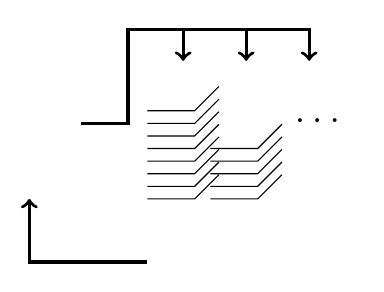
\begin{tikzpicture}[scale=0.8]
          \brick{1.25}{2}{Host}{gray}{}{}
          \begin{scope}[xshift=2.5cm,yshift=-1.5cm]
            \brick{2.5}{1.25}{Device}{gray}{}{}
          \end{scope}
          \begin{scope}[xshift=2.5cm]
            \brick{0.75}{2}{Queue 1}{blue}{text=white,rotate=90}{
              \foreach\i in {0,0.2,...,1.4}
                \draw (0,\i) -- (0.75,\i) -- (0.75,\i,-1);
            }
          \end{scope}
          \begin{scope}[xshift=3.5cm]
            \brick{0.75}{2}{Queue 2}{blue}{text=white,rotate=90}{
              \foreach\i in {0,0.2,...,0.9}
                \draw (0,\i) -- (0.75,\i) -- (0.75,\i,-1);
            }
          \end{scope}

          \node [font=\Large] at (5.25,1.25) {\dots} ;

          \draw [very thick,->] (1.25,1,-0.5) -| (2,2.5,-0.5) -| (2.875,2,-0.5);
          \draw [very thick,->] (2,2.5,-0.5) -| (3.875,2,-0.5);
          \draw [very thick,->] (2,2.5,-0.5) -| (4.875,2,-0.5);
          \draw [very thick,->] (2.5,-1) -| (0.625,0);
        \end{tikzpicture}
    \end{columns}
  \uncover<4->{
    \begin{tikzpicture} [overlay]
      \node [above left=1cm of current page.south east,draw,drop shadow,fill=white,
       inner sep=5mm,thick, text width=0.6\textwidth]
        {
          Important: Two different mechanisms at work!
        } ;
    \end{tikzpicture}
  }
  \end{frame}
}
% -----------------------------------------------------------------------------
\begin{frame}{Entertainment: GPU Memory Zoo}

  \uncover<+->{
    \begin{tabular}{p{5em}cccp{2.8cm}}
    \hline
    \textbf{Type} & \textbf{Per} & \textbf{Access} & \textbf{Latency} \\
    \hline
    \textbf<2->{private} & work item & R/W & 1 or 1000 \\
    \textbf<2->{local} & group & R/W & 2 \\
    \textbf<2->{global} & grid & R/W & 1000 & Cached?\\
    \texttt{constant} & grid & R/O & 1-1000 & Cached \\
    image$n$d\_t & grid & R(/W) & 1000 & Spatially cached\\
    \hline
    \end{tabular}
  }
\end{frame}
% -----------------------------------------------------------------------------
\subsection{Summary}
% -----------------------------------------------------------------------------
\begin{frame}{GPU performance summary}
  \begin{itemize}
    \item Latency, latency, latency!
      \begin{itemize}
        \item Various forms: Memory, branches, computation
        \item All need to be hidden
      \end{itemize}
    \item Bandwidth: usually fixable
    \item Watch your memory access patterns
      \begin{itemize}
        \item Local mem is somewhat more forgiving
        \item \dots and lower latency, higher BW
      \end{itemize}
  \end{itemize}
\end{frame}
\begin{frame}{Demo}
  \begin{center}
  \Huge GPU profiler demo
  \end{center}
\end{frame}

% }}}
% -----------------------------------------------------------------------------
\section{MPI performance}
% -----------------------------------------------------------------------------
% {{{
\begin{frame}{MPI}
  \begin{center}
  \Huge MPI performance demo
  \end{center}
\end{frame}
% }}}
% -----------------------------------------------------------------------------
\long\def\sectionslide#1#2#3#4{
  \begin{frame}
    \begin{center}
      {\Huge \textless #1
      {\fontsize{130}{150}\fontfamily{phv}\selectfont #2}
      \textgreater}

      \vspace{1.5cm}
      \textbf{#3}

      \medskip\footnotesize
      #4
    \end{center}
  \end{frame}
}
\sectionslide{/}{2}{Understanding Computational Cost}{}
\sectionslide{}{3}{Concepts, Patterns and Recipes}{}
% -----------------------------------------------------------------------------
\section{Parallel Patterns}
% -----------------------------------------------------------------------------
\begin{frame}{Patterns: Overview}
  Parallel Programming:
  \begin{itemize}
    \item To what problems does it apply?
    \item How?
      \subitem{How big of a headache?}
    \item What mechanism is suitable?
  \end{itemize}

  \bigskip
  Organize discussion by patterns of \textbf{Dependencies}.
  \uncover<+->{}
  \uncover<+->{
    \begin{tikzpicture} [overlay]
      \node [above left=1cm of current page.south east,draw,drop shadow,fill=white,
       inner sep=5mm,thick]
        {
          Will move to more of a \emph{discussion} style
        } ;
    \end{tikzpicture}
  }
\end{frame}
% -----------------------------------------------------------------------------
\subsection[Embarrassing]{Embarrassingly Parallel}
% -----------------------------------------------------------------------------
% {{{
\begin{frame}{Embarrassingly Parallel}
  \uncover<+>{}
  {\Huge
  \[
    y_i = f_i(x_i)
  \]}%
  where $i\in\{1,\dots,N\}$.

  \medskip
  Notation: (also for rest of this lecture)
  \begin{itemize}
    \item $x_i$: inputs
    \item $y_i$: outputs
    \item $f_i$: (pure) functions (i.e. \emph{no side effects})
  \end{itemize}

  \medskip
  \uncover<+>{
    \begin{tikzpicture} [overlay]
      \node [below left=1cm of current page.north east, draw,drop shadow,fill=white,
      text width=0.75\textwidth, inner xsep=0.5cm,inner ysep=0.5cm,thick]
        {
          When does a function have a ``side effect''?

          \bigskip
          In addition to producing a value, it
          \begin{itemize}
          \item modifies non-local state, or
          \item has an observable interaction with the outside world.
          \end{itemize}
        } ;
    \end{tikzpicture}
  }%
  \uncover<+(1)->{
  Often: $f_1=\dots=f_N$. Then
  \begin{itemize}
    \item Lisp/Python function \texttt{map}
    \item C++ STL \texttt{std::transform}
  \end{itemize}
  }
\end{frame}
% -----------------------------------------------------------------------------
\begin{frame}{Embarrassingly Parallel: Graph Representation}
  \begin{center}
    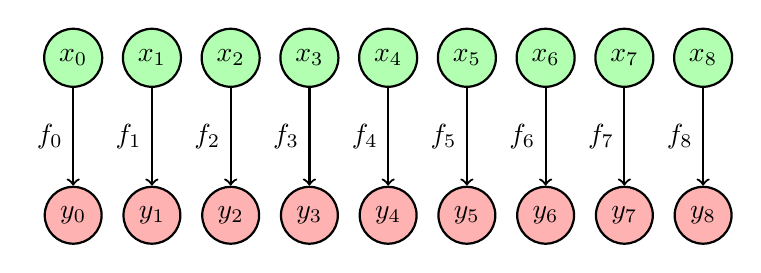
\begin{tikzpicture}
      \foreach \i in {0,1,...,8}
      {
        \node [input] at (\i, 0) (x\i) { $x_{\i}$ };
        \node [output] at (\i, -2) (y\i) { $y_{\i}$ };
        \draw [func] (x\i) -- (y\i) node [pos=0.5,anchor=east] {$f_{\i}$};
      }
    \end{tikzpicture}
  \end{center}
  \uncover<2>{
    \begin{tikzpicture} [overlay]
      \node [above left=1cm of current page.south east, draw,drop shadow,fill=white,
      text width=0.4\textwidth, inner xsep=0.5cm,inner ysep=0.5cm,thick]
        {
          Trivial? Often: no.
        } ;
    \end{tikzpicture}
  }
\end{frame}
% -----------------------------------------------------------------------------
\begin{frame}{Embarrassingly Parallel: Examples}
  \begin{columns}
    \column{0.6\textwidth}
      Surprisingly useful:
      \begin{itemize}
        \item Element-wise linear algebra:

          Addition, scalar
          multiplication (\emph{not} inner product)
        \item Image Processing: Shift, rotate, clip, scale, \dots
        \item Monte Carlo simulation
        \item (Brute-force) Optimization
        \item Random Number Generation
        \item Encryption, Compression

          (after blocking)
        \item Software compilation
          \subitem{\texttt{make -j8}}
      \end{itemize}
    \column{0.4\textwidth}
      \includegraphics[width=\textwidth]{parallel-field.jpeg}
  \end{columns}
  \uncover<2>{
    \begin{tikzpicture} [overlay]
      \node [above left=1cm of current page.south east, draw,drop shadow,fill=white,
      text width=0.5\textwidth, inner xsep=0.5cm,inner ysep=0.5cm,thick]
        {
          But: Still needs a minimum of coordination. How can that be
          achieved?
        } ;
    \end{tikzpicture}
  }
\end{frame}
\addimgcredit{Field: sxc.hu/mzacha}
% -----------------------------------------------------------------------------
\begin{frame}{Mapping to Mechanisms}
  \begin{itemize}[<+->]
    \item Single threads?
    \item OpenMP?
    \item MPI?
    \item MPI: Larger than \# ranks?
    \item GPU?
  \end{itemize}
\end{frame}
% -----------------------------------------------------------------------------
\begin{frame}{Mother-Child Parallelism}
  Mother-Child parallelism:

  \bigskip
  \begin{center}
  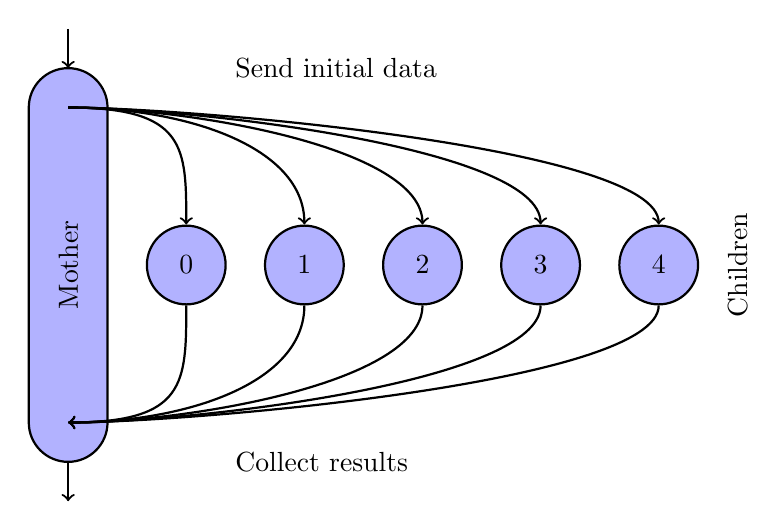
\begin{tikzpicture}
    \draw [rounded corners=0.5cm,thick,fill=intermed]
      (-0.5,2.5) rectangle (0.5,-2.5) ;
    \node [rotate=90] {Mother};

    \draw [func] (0,3) -- (0,2.5);
    \foreach \i in {0,...,4}
    {
      \node [circle,thick,fill=intermed,draw,thick,minimum height=1cm]
        (c\i) at (1.5+\i*1.5,0) {\i} ;
      \draw [func] (0,2) ..controls +(1.5,0) and +(0,1.5) .. (c\i);
      \draw [func] (c\i) ..controls +(0,-1.5) and +(1.5,0) .. (0,-2);
    }
    \node at(8.5,0) [rotate=90] {Children};
    \draw [func] (0,-2.5) -- (0,-3) ;
    \node at (2,2.5) [anchor=west] {Send initial data} ;
    \node at (2,-2.5) [anchor=west] {Collect results} ;
  \end{tikzpicture}
  \end{center}

  \bigskip
  (formerly called ``Master-Slave'')
\end{frame}
% -----------------------------------------------------------------------------
\begin{frame}{Embarrassingly Parallel: Issues}
  \begin{columns}
    \column{0.3\textwidth}
      \includegraphics[width=\textwidth]{question-mark.png}
    \column{0.6\textwidth}
      \begin{itemize}
        \item Process Creation:

          Dynamic/Static?
          \begin{itemize}
            \item MPI 2 supports dynamic process creation
          \end{itemize}
        \item Job Assignment (`Scheduling'):

          Dynamic/Static?
        \item Operations/data light- or heavy-weight?
        \item Variable-size data?
        \item Load Balancing:
          \subitem{Here: easy}
      \end{itemize}
  \end{columns}
  \uncover<2>{
    \begin{tikzpicture} [overlay]
      \node [above left=1cm of current page.south east, draw,drop shadow,fill=white,
      text width=0.4\textwidth, inner xsep=0.5cm,inner ysep=0.5cm,thick]
        {
          Can you think of a load balancing recipe?
        } ;
    \end{tikzpicture}
  }
\end{frame}
% }}}
% -----------------------------------------------------------------------------
\subsection{Partition}
% -----------------------------------------------------------------------------
% {{{
\begin{frame}{Partition}
  {\Huge
  \[
    y_i = f_i(x_{i-1}, x_i, x_{i+1})
  \]}
  where $i\in\{1,\dots,N\}$.

  \pause
  \bigskip
  Includes straightforward
  generalizations to dependencies on a larger (but
  not $O(P)$-sized!) set of neighbor inputs.

  \pause
  \bigskip
  \textbf{Point:} Processor $i$ \emph{owns} $x_i$. (``owns'' = is
  ``responsible for updating'')
\end{frame}
% -----------------------------------------------------------------------------
\begin{frame}{Partition: Graph}
  \begin{center}
    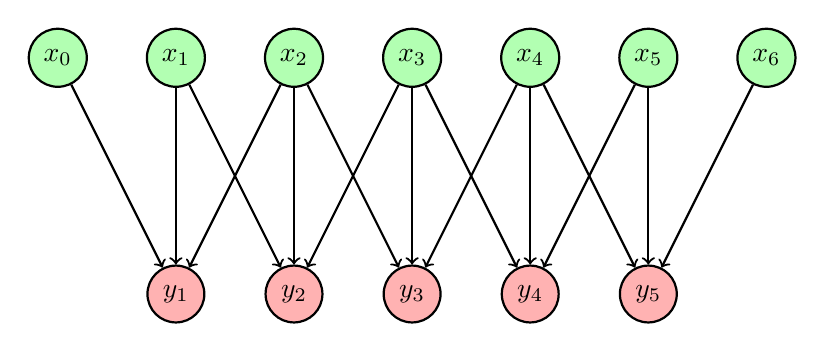
\begin{tikzpicture}
      \foreach \i in {0,...,6}
      {
        \node [input] at (1.5*\i, 0) (x\i) { $x_{\i}$ };
      }
      \foreach \i in {1,...,5}
      {
        \node [output] at (1.5*\i, -3) (y\i) { $y_{\i}$ };
      }
      \foreach \i in {1,...,5}
      {
        \pgfmathtruncatemacro{\iminusone}{\i-1}
        \pgfmathtruncatemacro{\iplusone}{\i+1}
        \draw [func] (x\i) -- (y\i) ;
        \draw [func] (x\iminusone) -- (y\i) ;
        \draw [func] (x\iplusone) -- (y\i) ;
      }
    \end{tikzpicture}
  \end{center}
\end{frame}
% -----------------------------------------------------------------------------
\begin{frame}{Mapping to Mechanisms}
  \begin{itemize}[<+->]
    \item OpenMP?
    \item MPI?
    \item MPI: Larger than \# ranks?
    \item GPU?
  \end{itemize}
\end{frame}
% -----------------------------------------------------------------------------
\begin{frame}{Partitioning for neighbor communication}
  \begin{center}
    \includegraphics[height=7cm]{mesh-partition.png}
  \end{center}
  \uncover<+>{}
  \uncover<+->{
    \begin{tikzpicture} [overlay]
      \node [above left=0.5cm of current page.south east, draw,drop shadow,fill=white,
      inner xsep=0.5cm,inner ysep=0.5cm,thick]
        {
          How can I chop up a domain?
        } ;
    \end{tikzpicture}
  }
\end{frame}
% -----------------------------------------------------------------------------
\begin{frame}{Mapping to Mechanisms: Stencils}
  \begin{columns}
    \column{0.5\textwidth}
      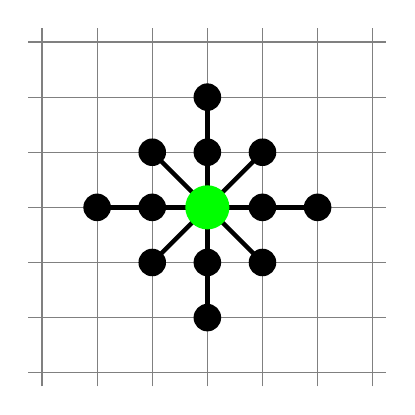
\begin{tikzpicture}[scale=0.7]
        \draw [black!50] (-0.25,-0.25) grid +(6.5,6.5);
        \foreach \i in {-2,...,2}
        {
          \fill (3+\i,3) circle (0.25);
          \fill (3,3+\i) circle (0.25);
        }
        \foreach \i in {-1,...,1}
        {
          \fill (3+\i,3+\i) circle (0.25);
          \fill (3-\i,3+\i) circle (0.25);
        }
        \draw [ultra thick] (3,3-2) -- ++ (0,4);
        \draw [ultra thick] (3-2,3) -- ++ (4,0);
        \draw [ultra thick] (3-1,3-1) -- ++ (2,2);
        \draw [ultra thick] (3-1,3+1) -- ++ (2,-2);

        \fill [green] (3,3) circle (0.4);
      \end{tikzpicture}
    \column{0.5\textwidth}


    Common example (``5-point stencil''):
    \begin{multline*}
      u^{n+1}_{i,j} =
        \frac{1}{h^2} (-4 u^n_{i,j}
        + u^n_{i-1,j}
        + u^n_{i+1,j}\\
        + u^n_{i,j-1}
        + u^n_{i,j+1})
    \end{multline*}

    \begin{itemize}[<+->]
      \item Sequential
      \item OpenMP?
      \item MPI?
      \item GPU --- 2D?
      \item GPU --- 3D?
    \end{itemize}
  \end{columns}
  \uncover<+>{}
  \uncover<+->{
    \begin{tikzpicture} [overlay]
      \node [above left=0.5cm of current page.south east, draw,drop shadow,fill=white,
      inner xsep=0.5cm,inner ysep=0.5cm,thick]
        {
          What if there's geometry?
        } ;
    \end{tikzpicture}
  }
\end{frame}
% -----------------------------------------------------------------------------
\begin{frame}{Partition: Issues}
  \begin{columns}
    \column{0.3\textwidth}
      \includegraphics[width=\textwidth]{question-mark.png}
    \column{0.6\textwidth}
      \begin{itemize}
        \item Only useful when the computation is mainly local
          \subitem{Responsibility for updating one datum
            rests with one processor}
        \item Synchronization, Deadlock, Livelock, \dots
          \begin{itemize}
            \item Performance Impact
            \item Granularity
          \end{itemize}
        \item Load Balancing: Thorny issue
          \subitem{$\rightarrow$ next lecture}
        \item Regularity of the Partition?
      \end{itemize}
  \end{columns}
\end{frame}
% -----------------------------------------------------------------------------
\begin{frame}{Rendezvous Trick}
  \begin{columns}
    \column{0.5\textwidth}
      \begin{itemize}
        \item Assume an irregular partition.
        \item Assume problem components $i$, $j$
        on unknown partitions $p_i$, $p_j$ need to communicate.
        \item How can $p_i$ find $p_j$ (and vice versa)?
      \end{itemize}

      \uncover<2->{
        Communicate via a\\ third party, $p_{f(i,j)}$.

        \medskip
        For $f$: think `hash function'.
      }

    \column{0.5\textwidth}
      \begin{tikzpicture}
        \node [circle,fill=intermed,minimum width=1.5cm,draw,thick]
          (pi) {$p_i$};
        \node [circle,below left=1cm and 1.5cm of pi,fill=intermed,
          minimum width=1.5cm,draw,thick]
          (pj) {$p_j$};
        \node [below=-0.6cm of pi, circle,fill=intermed,font=\small,draw,thick] (i) {$i$};
        \node [below=-0.6cm of pj, circle,fill=intermed,font=\small,draw,thick] (j) {$j$};
        \uncover<2->{
        \node [circle,below left=1.5cm and -0.6cm of pi,fill=green!30,
          minimum width=1.5cm,draw,thick]
          (med) {$p_{f(i,j)}$};
        }
        \uncover<3>{
          \draw [func] (i) -- (med)
            node [pos=0.5,anchor=west] {``I'm in $p_i$.''};
        }
        \uncover<4>{
          \draw [func] (j) -- (med)
            node [pos=0.7,anchor=west,rotate=75] {``I'm in $p_j$.''};
        }
        \uncover<6>{
          \draw [func] (med) -- (pj);
          \draw [func] (med) -- (pi);
        }
      \end{tikzpicture}
  \end{columns}
\end{frame}
% -----------------------------------------------------------------------------
\begin{frame}{Partition: Examples}
  \begin{columns}
    \column{0.7\textwidth}
      \begin{itemize}
        \item Time-marching

          (in particular: PDE solvers)
          \subitem{Including finite differences}
        \item Iterative Methods
          \begin{itemize}
            \item Solve $Ax=b$ (Jacobi, \dots)
            \item Optimization (all $P$ on single problem)
            \item Eigenvalue solvers
          \end{itemize}
        \item Cellular Automata (Game of Life :-)
      \end{itemize}
    \column{0.3\textwidth}
      \includegraphics[width=\textwidth]{voronoi-treemap.png}
  \end{columns}
\end{frame}
\addimgcredit{Voronoi Treemap: flickr.com/arenamontanus \cc }
% }}}
% -----------------------------------------------------------------------------
\subsection{Pipelines}
% -----------------------------------------------------------------------------
% {{{
\begin{frame}{Pipelined Computation}
  {\Huge
  \begin{align*}
    y = \;&f_N(\cdots f_2(f_1(x))\cdots ) \\
    =\; & (f_N \circ \cdots \circ f_1)(x)
  \end{align*}}
  where $N$ is fixed.
\end{frame}
% -----------------------------------------------------------------------------
\begin{frame}{Pipelined Computation: Graph}
  \begin{center}
    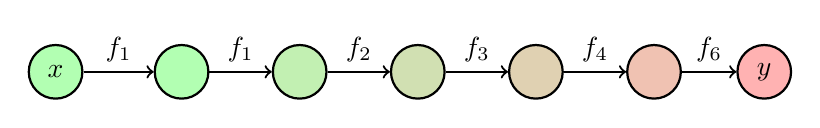
\begin{tikzpicture}
      \node [input] (x) { $x$ };
      \foreach \i in {0,...,4}
      {
        \pgfmathtruncatemacro{\blend}{\i*20}
        \node [input,fill=output!\blend!input] (m\i) at (1.6+\i*1.5,0) { \phantom{$x$} };
      }
      \node [output] (y) at (6*1.5,0) { $y$ };
      \draw [func] (x) -- (m0) node [pos=0.5,anchor=south] {$f_1$};
      \foreach \i in {0,...,3}
      {
        \pgfmathtruncatemacro{\iplusone}{\i+1}
        \draw [func] (m\i) -- (m\iplusone) node [pos=0.5,anchor=south] {$f_\iplusone$};
      }
      \draw [func] (m4) -- (y) node [pos=0.5,anchor=south] {$f_6$};
    \end{tikzpicture}
  \end{center}
  \uncover<2>{
    \begin{tikzpicture} [overlay]
      \node [above left=1cm of current page.south east, draw,drop shadow,fill=white,
      inner xsep=0.5cm,inner ysep=0.5cm,thick]
        {
          Processor Assignment?
        } ;
    \end{tikzpicture}
  }
\end{frame}
% -----------------------------------------------------------------------------
\begin{frame}{Pipelined Computation: Examples}
  \begin{columns}
    \column{0.6\textwidth}
      \begin{itemize}
        \item Image processing
        \item Any multi-stage algorithm
          \subitem{Pre/post-processing or I/O}
        \item Out-of-Core algorithms
      \end{itemize}

      \bigskip
      Specific simple examples:
      \begin{itemize}
        \item Sorting (insertion sort)
        \item Triangular linear system solve \\ (`backsubstitution')
          \subitem{Key: Pass on values as soon as they're available}
      \end{itemize}
      (will see more efficient algorithms for both later)
    \column{0.4\textwidth}
      \includegraphics[width=\textwidth]{pipe.jpeg}
  \end{columns}
\end{frame}
\addimgcredit{Pipe: sxc.hu/mterraza}
% -----------------------------------------------------------------------------
\begin{frame}{Pipelined Computation: Issues}
  \begin{columns}
    \column{0.3\textwidth}
      \includegraphics[width=\textwidth]{question-mark.png}
    \column{0.6\textwidth}
      \begin{itemize}
        \item Non-optimal while pipeline fills or empties
        \item Often communication-inefficient
          \subitem{for large data}
        \item Needs some attention to synchronization,
          deadlock avoidance
        \item Can accommodate some asynchrony

          But don't want:
          \begin{itemize}
            \item Pile-up
            \item Starvation
          \end{itemize}
      \end{itemize}
  \end{columns}
\end{frame}
% -----------------------------------------------------------------------------
\begin{frame}{Mapping to Mechanisms}
  \begin{itemize}[<+->]
    \item OpenMP?
    \item MPI?
    \item MPI: Larger than \# ranks?
    \item GPU?
  \end{itemize}
\end{frame}
% }}}
% -----------------------------------------------------------------------------
\subsection{Reduction}
% -----------------------------------------------------------------------------
% {{{
\begin{frame}{Reduction}
  {\Huge
  \[
    y =  f(\cdots f(f(x_1, x_2), x_3), \dots ,x_N)
  \]}
  where $N$ is the input size.

  \pause
  \medskip
  Also known as\dots
  \begin{itemize}
    \item Lisp/Python function \texttt{reduce} (Scheme: \texttt{fold})
    \item C++ STL \texttt{std::accumulate}
  \end{itemize}
\end{frame}

\begin{frame}{Reduction: Graph}
  \begin{center}
    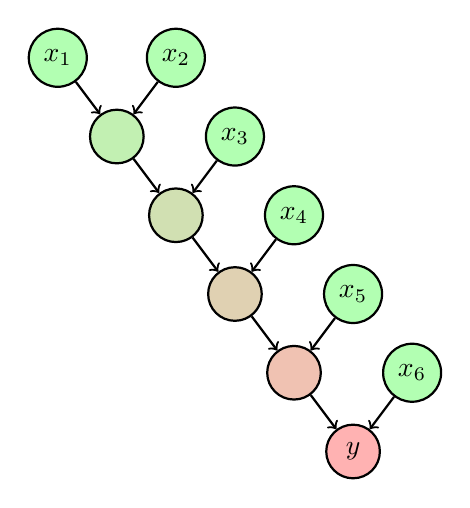
\begin{tikzpicture}[grow'=up,every path/.style={func,<-},level distance=1cm]
      \node [output] {$y$}
      child {
        node [input,fill=output!80!input] {}
        {
          child {
            node [input,fill=output!60!input] {}
            {
              child {
                node [input,fill=output!40!input] {}
                {
                  child {
                    node [input,fill=output!20!input] {}
                    {
                      child {node [input] {$x_1$} }
                      child {node [input] {$x_2$} }
                    }
                  }
                  child {node [input] {$x_3$} }
                }
              }
              child {node [input] {$x_4$} }
            }
          }
          child {node [input] {$x_5$} }
        }
      }
      child { node [input] {$x_6$} }
      ;
    \end{tikzpicture}
  \end{center}
  \uncover<2>{
    \begin{tikzpicture} [overlay]
      \node [above left=1cm of current page.south east, draw,drop shadow,fill=white,
      inner xsep=0.5cm,inner ysep=0.5cm,thick]
        {
          Painful! Not parallelizable.
        } ;
    \end{tikzpicture}
  }
\end{frame}
% -----------------------------------------------------------------------------
\begin{frame}{Approach to Reduction}
  \begin{columns}
    \column{0.4\textwidth}
      \tikz
        \node [rotate=40,font=\Huge\bfseries,
        cloud,cloud ignores aspect=true,cloud puffs=15,draw,thick]
        {{ $\mathit{f(x,y)}$?}};
    \column{0.6\textwidth}
      Can we do better?

      \medskip
      ``Tree'' very imbalanced. What property of $f$ would allow
      `rebalancing'?

      \pause
      \medskip
      \[
      f(f(x,y), z)=f(x,f(y,z))
      \]
      Looks less improbable if we let $x\circ y= f(x,y)$:
      \[
      x \circ(y\circ z))=(x \circ y) \circ z
      \]
      Has a very familiar name: \emph{Associativity}
  \end{columns}
\end{frame}
% -----------------------------------------------------------------------------
\begin{frame}{Reduction: A Better Graph}
  \begin{center}
    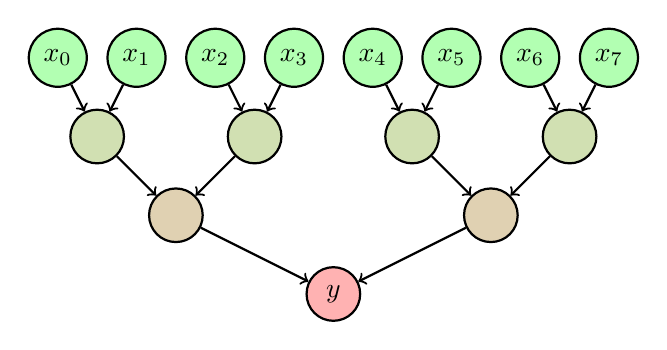
\begin{tikzpicture}[grow'=up,every path/.style={func,<-},level distance=1cm,
      level 1/.style={sibling distance=4cm},
      level 2/.style={sibling distance=2cm},
      level 3/.style={sibling distance=1cm},
      ]
      \node [output] {$y$}
      child {
        node [input,fill=output!60!input] {}
        child {
          node [input,fill=output!40!input] {}
          child { node [input] {$x_0$} }
          child { node [input] {$x_1$} }
        }
        child {
          node [input,fill=output!40!input] {}
          child { node [input] {$x_2$} }
          child { node [input] {$x_3$} }
        }
      }
      child {
        node [input,fill=output!60!input] {}
        child {
          node [input,fill=output!40!input] {}
          child { node [input] {$x_4$} }
          child { node [input] {$x_5$} }
        }
        child {
          node [input,fill=output!40!input] {}
          child { node [input] {$x_6$} }
          child { node [input] {$x_7$} }
        }
      }
      ;
    \end{tikzpicture}
  \end{center}
  \uncover<2>{
    \begin{tikzpicture} [overlay]
      \node [above right=1cm of current page.south west, draw,drop shadow,fill=white,
      inner xsep=0.5cm,inner ysep=0.5cm,thick]
        {
          Processor allocation?
        } ;
    \end{tikzpicture}
  }
\end{frame}
% -----------------------------------------------------------------------------
\begin{frame}{Mapping to Mechanisms}
  \begin{itemize}[<+->]
    \item Single threads?
    \item OpenMP?
    \item MPI?
    \item MPI: Larger than \# ranks?
    \item GPU?
  \end{itemize}
\end{frame}
% -----------------------------------------------------------------------------
\newcommand{\harriscredit}{
  \begin{tikzpicture}[overlay]
    \node [above left=1cm of current page.south east]
      [font=\scriptsize,fill=gray!30,opacity=0.8, text width=3.5cm]
      {With material by M.~Harris (Nvidia Corp.) };
  \end{tikzpicture}
}
\newcommand{\harrisred}[4]{

  \begin{frame}{#1}
    \includegraphics[viewport=0.5in #3 11in 7in,clip=true,page=#2,width=\textwidth]{harris-cuda-reduction.pdf}

    #4

    \harriscredit
  \end{frame}
}
% -----------------------------------------------------------------------------
\begin{frame}{Mapping Reduction to the GPU}
  \begin{itemize}
    \item<+-> Obvious: Want to use tree-based approach.
    \item Problem: Two scales, Work group and Grid
      \subitem{Need to occupy both to make good use of the machine.}
    \item In particular, need synchronization after each tree stage.
    \item<+-> Solution: Use a two-scale algorithm.
  \end{itemize}
  \uncover<.->{
  \includegraphics[viewport=0.5in 3in 9in 5.5in,clip=true,page=5,width=\textwidth]{harris-cuda-reduction.pdf}

  \emph{In particular:} Use multiple grid invocations to achieve
  inter-workgroup synchronization.
  }
  \harriscredit
\end{frame}
% -----------------------------------------------------------------------------
\begin{frame}{Kernel V1}
  \lstinputlisting[basicstyle=\footnotesize,linerange=red0-end]{oclReduction_kernel.cl}
\end{frame}
\harrisred{Interleaved Addressing}{8}{1.25in}{
  \setcounter{beamerpauses}{2}
  \uncover<+->{\textbf{Issue:} Slow modulo, Divergence}
}
% -----------------------------------------------------------------------------
\begin{frame}{Kernel V2}
  \lstinputlisting[basicstyle=\footnotesize,linerange=red2-end]{oclReduction_kernel.cl}
\end{frame}
\harrisred{Sequential Addressing}{14}{1.25in}{
  \setcounter{beamerpauses}{2}
  \uncover<+->{\textbf{Better!} But still not ``efficient''.\\[1ex]
  Only half of all work items after first round, \\ then a quarter, \dots}
}
% -----------------------------------------------------------------------------
\begin{frame}{Recap: Parallel Complexity}
  Distinguish:
  \begin{itemize}
    \item Time on $T$ processors: $T_P$
    \item \textbf{Step Complexity/Span} $T_\infty$: Minimum number of steps taken if
    an infinite number of processors are available
    \item Work per step $S_t$
    \item \textbf{Work Complexity/Work} $T_1=\sum_{t=1}^{T_\infty} S_t$: Total number of operations performed
    \item \textbf{Parallelism} $T_1/T_\infty$: average amount of work
    along span
      \subitem{$P>T_1/T_\infty$ doesn't make sense.}
  \end{itemize}
  Algorithm-specific!
\end{frame}
% -----------------------------------------------------------------------------
\begin{frame}{Parallel Complexity for Reduction}
  Number of Items $N$

  Actual work to be done: $W=O(N)$ additions.

  \medskip
  Step Complexity: Let $d=\lceil \log_2 N\rceil$.
  Then $T_\infty=d$, $S_t=O(2^{d-t})$.

  \medskip
  Work Complexity:
  \[
    T_1 = \sum_{t=1}^T S_t = O\left(\sum_{t=1}^T 2^{d-t}\right)
    = O(2^d)=O(N)
  \]
  \pause
  ``Work-efficient:'' $T_1 \sim W$.
\end{frame}
% -----------------------------------------------------------------------------
\begin{frame}{Greedy Scheduling}
  \begin{block}{Theorem (Graham `68, Brent `75)}
  A parallel algorithm with span $T_\infty$ and work complexity
  $T_1$ can be executed on a shared-memory machine with $P$ processors
  in no more than
  \[
    T_P \le \frac {T_1}P+T_\infty
  \]
  steps.
  \end{block}
  \bigskip
  Observations:
  \begin{itemize}
    \item Think of $T_\infty$ as the length of the ``critical path''.
    \item The first summand can be made to go away by increasing $P$.
    \item Only valid for shared-memory.
  \end{itemize}
  \uncover<2>{
    \begin{tikzpicture} [overlay]
      \node [above left=1cm of current page.south east, draw,drop shadow,fill=white,
      text width=0.5\textwidth, inner sep=0.5cm,thick]
        {
          Estimate for $P=1$?

          \medskip
          Proof sketch?
        } ;
    \end{tikzpicture}
  }
\end{frame}
% -----------------------------------------------------------------------------
\begin{frame}{Brent for Reduction}
  Again: Number of items $N$.

  \medskip
  Brent says
  \[
    T_P = O\left( \frac {T_1} P + T_\infty\right)
    = O\left( \frac N P + \log N\right).
  \]
  Within a work group: $N=P$ $\Rightarrow$ $T_N=O(\log N)$.

  \pause
  \bigskip
  But: Work groups are an illusion! Machine has finite width.

  Thus $T_P > O(\log N)$! How low can we take $P$ before we hurt
  our asymptotic runtime $T_P$?

  \pause
  \medskip
  Asymptotically optimal $T_P=O(\log N)$ for
  \[
  P \ge \frac N {\log N}.
  \]
  \textbf{Result:} We're free to reduce $P$ by a factor of $(\log N)$
  without increasing $T_P$. $\Rightarrow$ Do $(\log N)$ items in
  sequence per work item without increasing asymptotic $T_P$.
  \uncover<+(1)->{
    \begin{tikzpicture} [overlay]
      \node [below left=1cm of current page.north east, draw,drop shadow,fill=white,
      text width=0.6\textwidth, inner xsep=0.5cm,inner ysep=0.5cm,thick]
        {
          Think of this in terms of cost:
          \[
            \text{Cost}= P \times T_P
          \]%
          \only<+(1)->{%
          Brent gives lower bound on $P$.\\[1ex]
          Fewer Processors $\Rightarrow$ less cost!\\[1ex]
          \only<+(1)>{%
          ``\emph{Algorithm cascading}''
          }
          }%
        } ;
    \end{tikzpicture}
  }
\end{frame}
% -----------------------------------------------------------------------------
\begin{frame}{Kernel V3 Part 1}
  \lstinputlisting[basicstyle=\footnotesize,linerange=red6p1-end]{oclReduction_kernel.cl}
\end{frame}
% -----------------------------------------------------------------------------
\begin{frame}{Kernel V3 Part 2}
  \lstinputlisting[basicstyle=\footnotesize,linerange=red6p2-end]{oclReduction_kernel.cl}
\end{frame}
% -----------------------------------------------------------------------------
\harrisred{Performance Comparison}{36}{1.25in}{}
% -----------------------------------------------------------------------------
\begin{frame}{Reduction: Examples}
  \begin{columns}
    \column{0.6\textwidth}
      \begin{itemize}
        \item Sum, Inner Product, Norm
          \subitem{Occurs in iterative methods}
        \item Minimum, Maximum
        \item Data Analysis
          \subitem{Evaluation of Monte Carlo Simulations}
        \item List Concatenation, Set Union
        \item Matrix-Vector product (but\dots)
      \end{itemize}
    \column{0.4\textwidth}
      \includegraphics[width=\textwidth]{tree.jpeg}
  \end{columns}
\end{frame}
\addimgcredit{Tree: sxc.hu/bertvthul}
% -----------------------------------------------------------------------------
\begin{frame}{Reduction: Issues}
  \begin{columns}
    \column{0.3\textwidth}
      \includegraphics[width=\textwidth]{question-mark.png}
    \column{0.6\textwidth}
      \begin{itemize}
        \item When adding: floating point cancellation?
        \item Serial order goes faster:\\ can use registers for intermediate results
        \item Requires availability of neutral element
        \item GPU-Reduce: Optimization sensitive to data type
      \end{itemize}
  \end{columns}
\end{frame}
% }}}
% -----------------------------------------------------------------------------
\subsection{Map-Reduce}
% -----------------------------------------------------------------------------
% {{{
\begin{frame}{Map-Reduce}
  Sounds like this:
  {\Huge
  \begin{multline*}
    y =  f(\cdots f(f(g(x_1), g(x_2)), \\
      g(x_3)), \dots ,g(x_N))
  \end{multline*}
  }
  where $N$ is the input size.

  \begin{itemize}
    \item Lisp naming, again
    \item Mild generalization of reduction
  \end{itemize}
  \uncover<2->{
    \begin{tikzpicture} [overlay]
      \node [below left=1cm of current page.north east, draw,drop shadow,fill=white,
       inner xsep=0.5cm,inner ysep=0.5cm,thick]
        {
          But no. Not even close.
        } ;
    \end{tikzpicture}
  }
\end{frame}
% -----------------------------------------------------------------------------
\begin{frame}{Map-Reduce: Graph}
  \begin{center}
    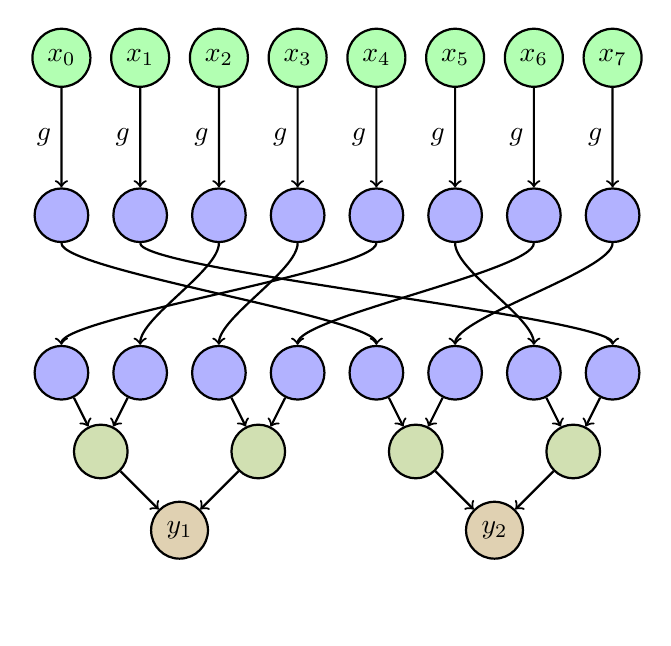
\begin{tikzpicture}[grow'=up,level distance=1cm,
      level 1/.style={sibling distance=4cm},
      level 2/.style={sibling distance=2cm},
      level 3/.style={sibling distance=1cm},
      level 4/.style={level distance=2cm,},
      every path/.style={func,<-},
      gfunc/.style={<-,
        edge from parent path={
          (\tikzparentnode\tikzparentanchor) --
          (\tikzchildnode\tikzchildanchor) node [left] {$g$}}
        },
      noarrow/.style={arrows=-,edge from parent path={}},
      doarrow/.style={<-,
        edge from parent path={
          (\tikzparentnode\tikzparentanchor) --
          (\tikzchildnode\tikzchildanchor) }
        },
      intermed/.style={input,fill=intermed},
      ]
      \node {}
      child [noarrow] {
        node [input,fill=output!60!input] {$y_1$}
        child [doarrow] {
          node [input,fill=output!40!input] {}
          child { node [intermed] (sgx0) {} child [noarrow] { node [intermed] (gx0) {} child [gfunc] {node [input] {$x_0$} } } }
          child { node [intermed] (sgx1) {} child [noarrow] { node [intermed] (gx1) {} child [gfunc] {node [input] {$x_1$} } } }
        }
        child [doarrow] {
          node [input,fill=output!40!input] {}
          child { node [intermed] (sgx2) {} child [noarrow] { node [intermed] (gx2) {} child [gfunc] {node [input] {$x_2$} } } }
          child { node [intermed] (sgx3) {} child [noarrow] { node [intermed] (gx3) {} child [gfunc] {node [input] {$x_3$} } } }
        }
      }
      child [noarrow] {
        node [input,fill=output!60!input] {$y_2$}
        child [doarrow] {
          node [input,fill=output!40!input] {}
          child { node [intermed] (sgx4) {} child [noarrow] { node [intermed] (gx4) {} child [gfunc] {node [input] {$x_4$} } } }
          child { node [intermed] (sgx5) {} child [noarrow] { node [intermed] (gx5) {} child [gfunc] {node [input] {$x_5$} } } }
        }
        child [doarrow] {
          node [input,fill=output!40!input] {}
          child { node [intermed] (sgx6) {} child [noarrow] { node [intermed] (gx6) {} child [gfunc] {node [input] {$x_6$} } } }
          child { node [intermed] (sgx7) {} child [noarrow] { node [intermed] (gx7) {} child [gfunc] {node [input] {$x_7$} } } }
        }
      }
      ;
      \draw [thick,->] (gx0) ..controls +(0,-7mm) and +(0,7mm).. (sgx4);
      \draw [thick,->] (gx1) ..controls +(0,-7mm) and +(0,7mm).. (sgx7);
      \draw [thick,->] (gx2) ..controls +(0,-7mm) and +(0,7mm).. (sgx1);
      \draw [thick,->] (gx3) ..controls +(0,-7mm) and +(0,7mm).. (sgx2);
      \draw [thick,->] (gx4) ..controls +(0,-7mm) and +(0,7mm).. (sgx0);
      \draw [thick,->] (gx5) ..controls +(0,-7mm) and +(0,7mm).. (sgx6);
      \draw [thick,->] (gx6) ..controls +(0,-7mm) and +(0,7mm).. (sgx3);
      \draw [thick,->] (gx7) ..controls +(0,-7mm) and +(0,7mm).. (sgx5);
    \end{tikzpicture}
  \end{center}
\end{frame}
% -----------------------------------------------------------------------------
\begin{frame}{MapReduce: Discussion}
  \begin{columns}
    \column{0.75\textwidth}
      MapReduce $\ge$ \texttt{map} $+$ \texttt{reduce}:

      \begin{itemize}
        \item Used by Google (and many others) for large-scale data
          processing
        \item Map generates $(\texttt{key},\texttt{value})$ pairs
          \begin{itemize}
            \item Reduce operates only on pairs with \emph{identical~keys}
            \item Remaining output sorted by key
          \end{itemize}
        \item Represent all data as character strings
          \subitem{User must convert to/from internal repr.}
        \item Messy implementation
          \subitem{Parallelization, fault tolerance,
            monitoring, data management, load balance, re-run
            ``stragglers'', data locality}
        \item Works for Internet-size data
        \item Simple to use even for inexperienced users
      \end{itemize}
    \column{0.2\textwidth}
      \includegraphics[height=\textwidth,angle=-90]{google-logo.png}
  \end{columns}
\end{frame}
% -----------------------------------------------------------------------------
\begin{frame}{MapReduce: Examples}
  \begin{columns}
    \column{0.2\textwidth}
      \includegraphics[height=\textwidth,angle=90]{google-logo.png}
    \column{0.8\textwidth}
      \begin{itemize}
        \item String search
        \item (e.g. URL) Hit count from Log
        \item Reverse web-link graph
          \subitem{desired: $(\texttt{target URL},\texttt{sources})$}
        \item Sort
        \item Indexing
          \subitem{desired: $(\texttt{word},\texttt{document IDs})$}
        \item Machine Learning, Clustering, \dots
      \end{itemize}
  \end{columns}
\end{frame}
% }}}
% -----------------------------------------------------------------------------
\subsection{Scan}
% -----------------------------------------------------------------------------
% {{{
\begin{frame}{Scan}
  {\Huge
  \begin{align*}
    y_1 &= x_1 \\
    y_2 &= f(y_1, x_2)\\
    \vdots &= \vdots \\
    y_N &= f(y_{N-1}, x_N)
  \end{align*}}
  where $N$ is the input size.

  \begin{itemize}
    \item Also called ``prefix sum''.
    \item Or cumulative sum (`\texttt{cumsum}') by Matlab/NumPy.
  \end{itemize}
\end{frame}
% -----------------------------------------------------------------------------
\begin{frame}{Scan: Graph}
  \begin{center}
    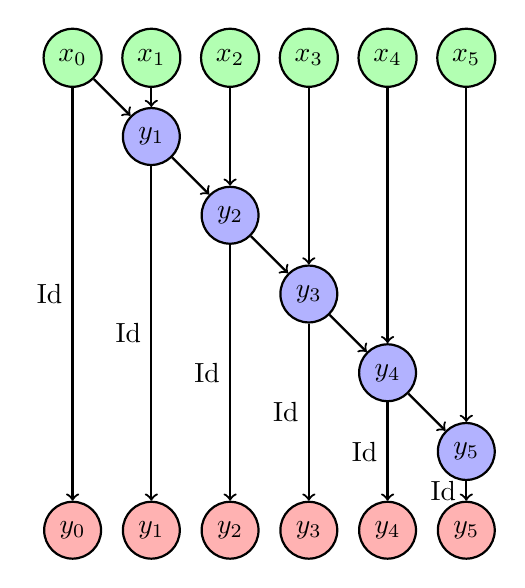
\begin{tikzpicture}[
      intermed/.style={input,fill=intermed},
      ffunc/.style={func,
        execute at end to={ node [left] {$f$}}
        },
      ]
      \foreach \i in {0,1,...,5}
      {
        \node [input] at (\i, 0) (x\i) { $x_{\i}$ };
        \node [output] at (\i, -6) (y\i) { $y_{\i}$ };
      }
      \foreach \i in {1,...,5}
      {
        \pgfmathtruncatemacro{\iminusone}{\i-1}
        \node [intermed] at (\i, -\i) (m\i) { $y_{\i}$ };
        \draw [func] (m\i) -- (y\i) node [pos=0.5,anchor=east] {Id};
        \draw [func] (x\i) -- (m\i) ;
      }
      \foreach \i in {2,...,5}
      {
        \pgfmathtruncatemacro{\iminusone}{\i-1}
        \draw [func] (m\iminusone) -- (m\i) ;
      }
      \draw [ffunc] (x0) -- (m1) ;
      \draw [func] (x0) -- (y0) node [pos=0.5,anchor=east] {Id};
    \end{tikzpicture}
  \end{center}
  \uncover<2->{
    \begin{tikzpicture} [overlay]
      \node [below left=1cm of current page.north east, draw,drop shadow,fill=white,
      text width=0.6\textwidth, inner xsep=0.5cm,inner ysep=0.5cm,thick]
        {
          This can't possibly be parallelized.

          Or can it?

          \only<3>{Again: Need assumptions on $f$.\\
          Associativity, commutativity.}
        } ;
    \end{tikzpicture}
  }
\end{frame}
% -----------------------------------------------------------------------------
\begin{frame}{Scan: Implementation}
  \begin{center}
    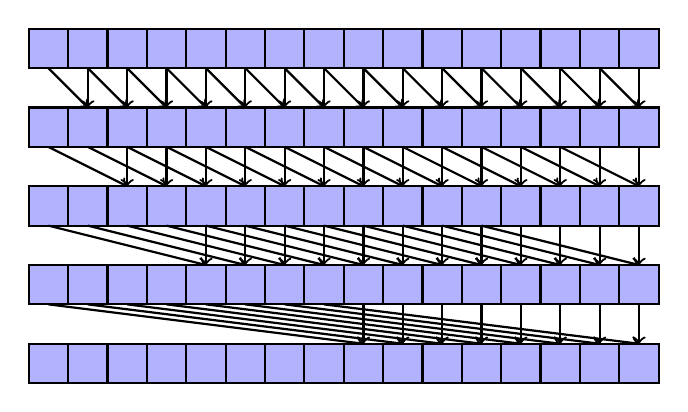
\begin{tikzpicture}[y=-1cm,scale=0.5]
      \foreach \i in {0,...,4}
      {
        \pgfmathtruncatemacro{\pwr}{2^\i}
        \pgfmathtruncatemacro{\nmpwr}{15-\pwr}
        \foreach \j in {0,...,15}
          \draw [fill=intermed,thick,draw] (\j,2*\i) rectangle +(1,1);
        \ifthenelse{\equal{\i}{4}}{}{
          \foreach \j in {\pwr,...,15}
            \draw [func] (\j,2*\i) ++(0.5,1) -- ++(0,1);
          \foreach \j in {0,...,\nmpwr}
            \draw [func] (\j,2*\i) ++(0.5,1) -- ++(\pwr,1);
        }
      }
    \end{tikzpicture}
  \end{center}
  \uncover<2->{
    \begin{tikzpicture} [overlay]
      \node [above left=1cm of current page.south east, draw,drop shadow,fill=white,
      inner xsep=0.5cm,inner ysep=0.5cm,thick]
        {
          Work-efficient?
        } ;
    \end{tikzpicture}
  }
\end{frame}
% -----------------------------------------------------------------------------
\begin{frame}{Scan: Implementation II}
  \begin{columns}
    \column{0.7\textwidth}
      Two sweeps: Upward, downward, \\
      both tree-shape

      \bigskip
      On upward sweep:
      \begin{itemize}
        \item Get values \texttt{L} and \texttt{R} from left and right child
        \item Save $L$ in local variable \texttt{Mine}
        \item Compute $\texttt{Tmp}=\texttt{L}+\texttt{R}$
          and pass to parent
      \end{itemize}

      On downward sweep:
      \begin{itemize}
        \item Get value $\texttt{Tmp}$ from parent
        \item Send $\texttt{Tmp}$ to left child
        \item Sent $\texttt{Tmp+Mine}$ to right child
      \end{itemize}
    \column{0.3\textwidth}
      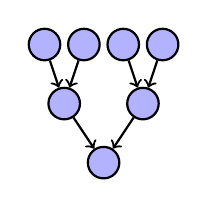
\begin{tikzpicture}[
      grow=up,
      every node/.style={circle,fill=intermed,draw,thick, minimum width=0.4cm},
      every path/.style={func,<-},
      level distance=0.75cm,
      level 1/.style={sibling distance=1cm},
      level 2/.style={sibling distance=0.5cm},
      ]
        \node {}
        child {
          node {}
          child { node {} }
          child { node {} }
        }
        child {
          node {}
          child { node {} }
          child { node {} }
        }
        ;
      \end{tikzpicture}

      \bigskip
      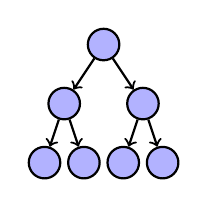
\begin{tikzpicture}[
      grow=down,
      every node/.style={circle,fill=intermed,draw,thick, minimum width=0.4cm},
      every path/.style={func,->},
      level distance=0.75cm,
      level 1/.style={sibling distance=1cm},
      level 2/.style={sibling distance=0.5cm},
      ]
        \node {}
        child {
          node {}
          child { node {} }
          child { node {} }
        }
        child {
          node {}
          child { node {} }
          child { node {} }
        }
        ;
      \end{tikzpicture}
  \end{columns}
  \uncover<2->{
    \begin{tikzpicture} [overlay]
      \node [above left=1cm of current page.south east, draw,drop shadow,fill=white,
      text width=0.6\textwidth,inner xsep=0.5cm,inner ysep=0.5cm,thick]
        {
          Work-efficient?

          Span rel. to first attempt?
        } ;
    \end{tikzpicture}
  }
\end{frame}
% -----------------------------------------------------------------------------
\begin{frame}{Scan: Examples}
  \begin{columns}
    \column{0.6\textwidth}
      \begin{itemize}
        \item Anything with a loop-carried dependence
        \item One row of Gauss-Seidel
        \item One row of triangular solve
        \item Segment numbering if boundaries are known
        \item Low-level building block for many higher-level algorithms
        algorithms
        \item FIR/IIR Filtering
        \item G.E.~Blelloch:
        \weblink{http://www.cs.cmu.edu/~guyb/papers/Ble93.pdf}{Prefix Sums and their Applications}
      \end{itemize}

    \column{0.3\textwidth}
      \includegraphics[width=\textwidth]{radar.png}
  \end{columns}
\end{frame}
\addimgcredit{Radar: sxc.hu/KimPouss}
% -----------------------------------------------------------------------------
\begin{frame}{Scan: Issues}
  \begin{columns}
    \column{0.3\textwidth}
      \includegraphics[width=\textwidth]{question-mark.png}
    \column{0.6\textwidth}
      \begin{itemize}
        \item Subtlety: Inclusive/Exclusive Scan
        \item Pattern sometimes hard to recognize
          \begin{itemize}
            \item But shows up surprisingly often
            \item Need to prove associativity/commutativity
          \end{itemize}
        \item Useful in Implementation: algorithm cascading
          \subitem{Do sequential scan on parts, then parallelize at
          coarser granularities}
      \end{itemize}
  \end{columns}
\end{frame}
% -----------------------------------------------------------------------------
\begin{frame}{Mapping to Mechanisms}
  \begin{itemize}[<+->]
    \item OpenMP?
    \item MPI?
    \item MPI: Larger than \# ranks?
    \item GPU?
  \end{itemize}
\end{frame}
% }}}
% -----------------------------------------------------------------------------
\subsection[D\&C]{Divide-and-Conquer}
% -----------------------------------------------------------------------------
% {{{
{
  \tikzset
  {
    sbrick/.style={rectangle split,rectangle split parts=#1,draw,thick,
      rectangle split allocate boxes=#1, rectangle split horizontal,
      anchor=west},
    ibrick/.style={sbrick=#1,fill=intermed!30!input},
    obrick/.style={sbrick=#1,fill=intermed!50!output},
  }
  \begin{frame}{Divide and Conquer}
    \begin{columns}
      \column{0.4\textwidth}
        {\huge
        \[
          y_i = f_i(x_1,\dots, x_N)
        \]}
        for $i\in\{1,dots,M\}$.

        \medskip
        \textbf{Main purpose:}
        A way of partitioning up fully dependent tasks.

      \column{0.5\textwidth}
        \begin{center}
          \begin{tikzpicture}[y=-0.8cm]
            \node [sbrick=8,fill=input] (l0/0) {
              $x_0$
              \nodepart{two} $x_1$
              \nodepart{three} $x_2$
              \nodepart{four} $x_3$
              \nodepart{five} $x_4$
              \nodepart{six} $x_5$
              \nodepart{seven} $x_6$
              \nodepart{eight} $x_7$
            };

            \node [ibrick=4,] (l1/0) at (-0.25,1) {
              $x_0$
              \nodepart{two} $x_1$
              \nodepart{three} $x_2$
              \nodepart{four} $x_3$
            };

            \node [ibrick=4,right=0.5cm of l1/0] (l1/1) {
              $x_4$
              \nodepart{two} $x_5$
              \nodepart{three} $x_6$
              \nodepart{four} $x_7$
            };

            \node [ibrick=2,] (l2/0) at (-0.45,2) {
              $x_0$ \nodepart{two} $x_1$
            };
            \node [ibrick=2,right=0.3cm of l2/0] (l2/1) {
              $x_2$ \nodepart{two} $x_3$
            };
            \node [ibrick=2,right=0.3cm of l2/1] (l2/2) {
              $x_4$ \nodepart{two} $x_5$
            };
            \node [ibrick=2,right=0.3cm of l2/2] (l2/3) {
              $x_6$ \nodepart{two} $x_7$
            };

            \node [obrick=2,] (l5/0) at (-0.55,5) {
              $u_0$ \nodepart{two} $u_1$
            };
            \node [obrick=2,right=0.3cm of l5/0] (l5/1) {
              $u_2$ \nodepart{two} $u_3$
            };
            \node [obrick=2,right=0.3cm of l5/1] (l5/2) {
              $u_4$ \nodepart{two} $u_5$
            };
            \node [obrick=2,right=0.3cm of l5/2] (l5/3) {
              $u_6$ \nodepart{two} $u_7$
            };

            \foreach\i in {0,...,7}
            {
              \node [fill=intermed!30!input,thick,draw,anchor=west] at (-0.45cm+\i*2em,3) (l3/\i) { $x_\i$ };
              \pgfmathtruncatemacro{\updiv}{\i/2}
              \draw [func] (l2/\updiv) -- (l3/\i) ;
              \node [fill=intermed,thick,draw,anchor=west] at (-0.45cm+\i*2em,4) (l4/\i) { $y_\i$ };
              \draw [func] (l3/\i) -- (l4/\i) ;
              \draw [func] (l4/\i) -- (l5/\updiv) ;
            }

            \node [obrick=4,] (l6/0) at (-0.25,6) {
              $v_0$
              \nodepart{two} $v_1$
              \nodepart{three} $v_2$
              \nodepart{four} $v_3$
            };

            \node [obrick=4,right=0.5cm of l6/0] (l6/1) {
              $v_4$
              \nodepart{two} $v_5$
              \nodepart{three} $v_6$
              \nodepart{four} $v_7$
            };

            \node [sbrick=8,fill=output] at (0,7) (l7/0) {
              $w_0$
              \nodepart{two} $w_1$
              \nodepart{three} $w_2$
              \nodepart{four} $w_3$
              \nodepart{five} $w_4$
              \nodepart{six} $w_5$
              \nodepart{seven} $w_6$
              \nodepart{eight} $w_7$
            };

            \draw [func] (l0/0) -- (l1/0);
            \draw [func] (l0/0) -- (l1/1);

            \draw [func] (l1/0) -- (l2/0);
            \draw [func] (l1/0) -- (l2/1);

            \draw [func] (l1/1) -- (l2/2);
            \draw [func] (l1/1) -- (l2/3);

            \draw [func] (l5/0) -- (l6/0);
            \draw [func] (l5/1) -- (l6/0);

            \draw [func] (l5/2) -- (l6/1);
            \draw [func] (l5/3) -- (l6/1);

            \draw [func] (l6/0) -- (l7/0);
            \draw [func] (l6/1) -- (l7/0);
          \end{tikzpicture}
        \end{center}
    \end{columns}
    \uncover<2>{
      \begin{tikzpicture} [overlay]
        \node [above right=1cm of current page.south west, draw,drop shadow,fill=white,
        inner xsep=0.5cm,inner ysep=0.5cm,thick]
          {
            Processor allocation?
          } ;
      \end{tikzpicture}
    }
  \end{frame}
}
% -----------------------------------------------------------------------------
\begin{frame}{Divide and Conquer: Examples}
  \begin{columns}
    \column{0.6\textwidth}
      \begin{itemize}
        \item GEMM, TRMM, TRSM, GETRF (LU)
        \item FFT
        \item Sorting: Bucket sort, Merge sort
        \item $N$-Body problems (Barnes-Hut, FMM)
        \item Adaptive Integration
      \end{itemize}

      More fun with work and span:
      \weblink{http://supertech.csail.mit.edu/cilk/lecture-2.pdf}{D\&C
      analysis lecture}

    \column{0.3\textwidth}
      \includegraphics[width=\textwidth]{quadtree.png}
  \end{columns}
\end{frame}

\addimgcredit{Quadtree: flickr.com/ethanhein \cc}
% -----------------------------------------------------------------------------
\begin{frame}{Mapping to Mechanisms}
  \begin{itemize}[<+->]
    \item OpenMP?
    \item MPI?
    \item MPI: Larger than \# ranks?
    \item GPU?
  \end{itemize}
\end{frame}
% -----------------------------------------------------------------------------
\begin{frame}{Divide and Conquer: Issues}
  \begin{columns}
    \column{0.3\textwidth}
      \includegraphics[width=\textwidth]{question-mark.png}
    \column{0.7\textwidth}
      \begin{itemize}
        \item ``No idea how to parallelize that''
          \subitem{$\rightarrow$ Try D\&C}
        \item Non-optimal during partition, merge
          \subitem{But: Does not matter if deep levels do heavy enough
          processing}
        \item Subtle to map to fixed-width machines (e.g. GPUs)
          \subitem{Varying data size along tree}
        \item Bookkeeping nontrivial for non-$2^n$ sizes
        \item Side benefit: D\&C is generally cache-friendly
      \end{itemize}
  \end{columns}
\end{frame}
% }}}
% -----------------------------------------------------------------------------
\subsection[General]{General Data Dependencies}
% -----------------------------------------------------------------------------
% {{{
\begin{frame}{General Dependency Graphs}
  \begin{columns}
    \column{0.3\textwidth}
      B = f(A)\\
      C = g(B)\\
      E = f(C)\\
      F = h(C)\\
      G = g(E,F)\\
      P = p(B)\\
      Q = q(B)\\
      R = r(G,P,Q)
    \column{0.6\textwidth}
      \begin{center}
        \input{general-dep-graph}
      \end{center}
  \end{columns}
  \uncover<2>{
    \begin{tikzpicture} [overlay]
      \node [above right=1cm of current page.south west, draw,drop shadow,fill=white,
      text width=0.6\textwidth, inner xsep=0.5cm,inner ysep=0.5cm,thick]
        {
          Great: All patterns discussed so far can be reduced to this one.
        } ;
    \end{tikzpicture}
  }
\end{frame}
% -----------------------------------------------------------------------------
\begin{frame}{Mapping to Mechanisms}
  \begin{itemize}[<+->]
    \item OpenMP?
    \item MPI?
    \item MPI: Larger than \# ranks?
    \item GPU?
  \end{itemize}
\end{frame}
% -----------------------------------------------------------------------------
\begin{frame}{Cilk}
  \begin{columns}
    \column{0.4\textwidth}
      \lstinputlisting{cilk-demo.c}
    \column{0.5\textwidth}
      Features:
      \begin{itemize}
        \item Adds keywords 
        \texttt{spawn}, \texttt{sync},
        (\texttt{inlet}, \texttt{abort})
        \item Remove keywords $\rightarrow$ valid (seq.) C
      \end{itemize}

      Timeline:
      \begin{itemize}
        \item Developed at MIT, starting in `94
        \item Commercialized in `06
        \item Bought by Intel in `09
        \item Available in the Intel Compilers
      \end{itemize}

  \end{columns}
  \uncover<2>{
    \begin{tikzpicture} [overlay]
      \node [above right=1cm of current page.south west, draw,drop shadow,fill=white,
      inner xsep=0.5cm,inner ysep=0.5cm,thick]
        {
          Efficient implementation?
        } ;
    \end{tikzpicture}
  }
\end{frame}
% -----------------------------------------------------------------------------
\newcommand{\cilkcredit}{
  \begin{tikzpicture}[overlay]
    \node [above left=1cm of current page.south east]
      [font=\scriptsize,fill=gray!30,opacity=0.8, text width=3.5cm]
      {With material by Charles~E.~Leiserson (MIT)};
  \end{tikzpicture}
}
\newcommand{\cilkslide}[3]{

  \begin{frame}{#1}
    
\includegraphics[viewport=0in 0.5in 11in 7.5in,clip=true,page=#2,width=\textwidth]{cilk-lec-1.pdf}

    \cilkcredit #3
  \end{frame}
}

\cilkslide{Work-Stealing}{46}{}
\cilkslide{Work-Stealing}{47}{}
\cilkslide{Work-Stealing}{48}{}
\cilkslide{Work-Stealing}{49}{}
\cilkslide{Work-Stealing}{50}{}
\cilkslide{Work-Stealing}{51}{}
\cilkslide{Work-Stealing}{52}{}
\cilkslide{Work-Stealing}{53}{%
  \uncover<2>{%
    \begin{tikzpicture} [overlay]
      \node [above right=1cm of current page.south west, draw,drop shadow,fill=white,
      text width=0.5\textwidth,inner sep=0.5cm,thick]
        { Why is Work-Stealing better than a Task Queue?  } ;
    \end{tikzpicture}%
  }
  
}
% -----------------------------------------------------------------------------
\begin{frame}{General Graphs: Issues}
  \begin{columns}
    \column{0.3\textwidth}
      \includegraphics[width=\textwidth]{question-mark.png}
    \column{0.7\textwidth}
      \begin{itemize}
        \item Model can accommodate `speculative execution'
          \begin{itemize}
            \item Launch many different `approaches'
            \item Abort the others as soon as one satisfactory one
            emerges.
          \end{itemize}

        \item Discover dependencies, make up schedule at run-time%
          \begin{itemize}
            \item Usually less efficient than the case of known
            dependencies
            \item Map-Reduce absorbs many cases that would otherwise
            be general
          \end{itemize}
        \item On-line scheduling: complicated
        \item Not a good fit if a more specific pattern applies
        \item Good if inputs/outputs/functions are (somewhat) heavy-weight
      \end{itemize}
  \end{columns}
\end{frame}
% }}}

% {{{

% - divide and conquer
% - General data deps: OpenCL events, OOO queues, partitioning,
%   implicit dependencies in CL
% - scan: design a sorting alg based on it

% }}}

\questionframe{}
\imagecreditslide

\end{document}
% vim: foldmethod=marker

